\documentclass[a4paper]{article}
\usepackage[utf8]{inputenc}
\usepackage{amsmath}
\usepackage{amssymb}
\usepackage{caption}
\usepackage{mathtools}
\usepackage{amsfonts}
\usepackage{lastpage}
\usepackage{tikz}
\usepackage{float}
\usepackage{textcomp}
\usetikzlibrary{patterns}
\usepackage{pdfpages}
\usepackage{gauss}
\usepackage{fancyvrb}
\usepackage[table]{colortbl}
\usepackage{fancyhdr}
\usepackage{graphicx}
\usepackage[margin=2.5 cm]{geometry}

\definecolor{listinggray}{gray}{0.9}
\usepackage{listings}
\lstset{
	language=,
	literate=
		{æ}{{\ae}}1
		{ø}{{\o}}1
		{å}{{\aa}}1
		{Æ}{{\AE}}1
		{Ø}{{\O}}1
		{Å}{{\AA}}1,
	backgroundcolor=\color{listinggray},
	tabsize=3,
	rulecolor=,
	basicstyle=\scriptsize,
	upquote=true,
	aboveskip={0.2\baselineskip},
	columns=fixed,
	showstringspaces=false,
	extendedchars=true,
	breaklines=true,
	prebreak =\raisebox{0ex}[0ex][0ex]{\ensuremath{\hookleftarrow}},
	frame=single,
	showtabs=false,
	showspaces=false,
	showlines=true,
	showstringspaces=false,
	identifierstyle=\ttfamily,
	keywordstyle=\color[rgb]{0,0,1},
	commentstyle=\color[rgb]{0.133,0.545,0.133},
	stringstyle=\color[rgb]{0.627,0.126,0.941},
  moredelim=**[is][\color{blue}]{@}{@},
}

\lstdefinestyle{base}{
  emptylines=1,
  breaklines=true,
  basicstyle=\ttfamily\color{black},
}

\pagestyle{fancy}
\def\checkmark{\tikz\fill[scale=0.4](0,.35) -- (.25,0) -- (1,.7) -- (.25,.15) -- cycle;}
\newcommand*\circled[1]{\tikz[baseline=(char.base)]{
            \node[shape=circle,draw,inner sep=2pt] (char) {#1};}}
\newcommand*\squared[1]{%
  \tikz[baseline=(R.base)]\node[draw,rectangle,inner sep=0.5pt](R) {#1};\!}
\newcommand{\comment}[1]{%
  \text{\phantom{(#1)}} \tag{#1}}
\def\el{[\![}
\def\er{]\!]}
\def\dpip{|\!|}
\def\MeanN{\frac{1}{N}\sum^N_{n=1}}
\cfoot{Page \thepage\ of \pageref{LastPage}}
\DeclareGraphicsExtensions{.pdf,.png,.jpg}
\author{Nikolaj Dybdahl Rathcke (rfq695)}
\title{Graph Coloring \\ Assignment 3}
\lhead{Graph Coloring}
\rhead{Assignment 3}

\begin{document}
\maketitle

\section{Problem 1}
Instead of computing the edge chromatic number for each "iteration" of the \texttt{FunnyGraph}, we can use a combination of Vizing's theorem and Preposition $3$ from the lecture notes (lecture 11). Vizing's theorem states that the edge chromatic number of a graph $G$ is always equal to $\Delta G$ (class one) or $\Delta+1$ (class two). Preposition $3$ from lecture notes $11$ states that if $G$ has only one vertex of maximal degree, then the chromatic index $\chi'$ is exactly $\Delta G$. \\
The first step of \texttt{FunnyGraph}, is to produce a complete graph on $n$ vertices and removes a cycle. This gives us a $n-3$ regular graph that we will call $FG$. This means that $\Delta FG=n-3$ as removing the cycle will decrease every degree of the graph by $2$. We then construct the Mycielski graph $FG'$ of $FG$, which changes the max degree to $2(n-3)$. This is pretty easy to see as the original vertices from $FG$ will be connected to an addition $n-3$ vertices in $FG'$ (the other vertices have degree at most $n-1$). Lastly, we join $FG'$ with the wheel graph $W_{n+1}$ to get $FG''$. All the original vertices from $FG$ then have degree:
$$
2(n-3)+n+1=3n-5
$$
The center vertex in the wheel graph, however, will be connected to the entire mycielski graph $FG'$ and $n$ vertices in the wheel graph. This will give that vertex a degree of:
$$
2n+1+n=3n+1
$$
Which is the max degree in the graph. Now using Vizing's theorem, we know the \texttt{FunnyGraph} on $n$ vertices has a chromatic index of $3n+1$ or $3n+2$. But since the the center vertex is the only vertex of maximal degree, we can use Preposition $3$ to conclude that the \texttt{FunnyGraph} has chromatic index $3n+1$. Thus, we can find the chromatic index of \texttt{FunnyGraph} on $99$ vertices:
$$
3\cdot 99+1=298
$$
Which means we need $298$ colors so that no adjacent edges are colored the same.

\section{Problem 2}
\subsection{(a)}
If we have a vector of scalars $a_1,a_2,..,a_d$. Then from the definition of a hyperplane, we have that the set of vectors
$$
\begin{bmatrix}
x_1 \\
x_2 \\
\vdots \\
x_d
\end{bmatrix}
$$
in $\mathbb{R}^d$ that satisfies the equation
$$
a_1x_1+a_2x_2+\dots+a_dx_d = c
$$
for some constant $c$ is the hyperplane. Since we can set all scalars to $1$, then we can easily realize that the unit distance graph $Q_d(u,s)$ (Lemma $13$ from lecture notes $12$ states that all $Q_d(u)$ are unit graphs) is in the hyperplane to the unit distance graph $Q_d$ since $c=s$ for all values of $s$. A hyperplane is by definition the subspace of one dimension less that its ambient space, so $Q_d(u,s)$ is in $\mathbb{R}^{d-1}$.

\subsection{(b)}
We want to use bound:
$$
\chi(\mathbb{R}^d)\geq \chi(Q_{10}(u,s)\geq \frac{|Q_{10}(u,s)|}{\alpha(Q_{10}(u,s)}
$$
Obviously, we want to find the independence number of some graph that maximizes the rightmost expression. This can be computed in Sage by brute-force. That is, we try all the combinations of $u$ and $s$ and see which one produces the largest value. This is shown to be when $u=4$ and $s=5$, which gives us an independece number of $12$ and a bound on $21$. This means we can say
$$
\chi(\mathbb{R}^9)\geq 21
$$
which is the best bound we can get. We could try to compute the chromatic number of $Q_{10}(u,s)$ since we are using brute force. But the chromatic number is actually a lot heavier to compute even though both the chromatic number and maximal independent set are both NP-hard problems.

\section{Problem 3}
If we look at the coloring in one dimension, imagine a coloring where we a pick a point $x\in \mathbb{R}$. We then color the points $x-1$ and $x+1$ with another color (an do this to infinity by alternating the colors). Now this ensures that any finite graph $G$ can be colored with two colors in $1$ dimension, but it can be a little hard to see how it works on the entirety of $\mathbb{R}$. We can use Theorem $9$ from lecture notes $11$, which states that if every \textit{finite} subgraph of a graph $G$ can be colored with $k$ colors, then $G$ can be colored with $k$ colors. This means we can color one dimension with $2$ colors. \\
If now we extend it to $2$ dimensions, it is the same problem with one dimension more. So for any of the colors we used in $\mathbb{R}$, we need an additional (new) color in $\mathbb{R}^2$ to ensure that there is no conflict in the new dimension when we use the same strategy of coloring. This means we actually need $2^d$ colors to correctly color $\mathbb{R}^d$. \\
Now we need to show that this solution is in fact optimal. To see this, consider the unit hypercube in dimension $d$. It has exactly $2^d$ points. All of them has a supremum metric of $1$ to each other, since they cannot differ in value by more than $1$ in any dimension and any two points will always differ by $1$ in at least one dimension. This means all $2^d$ points must be colored with different colors, so it is a lower bound to the coloring of $\mathbb{R}^d$, and thus the proposed coloring using $2^d$ colors must be optimal.

\section{Problem 4}
If we consider the case where $n=2$, we can pick any edge (the red in Figure \ref{fig1}) and color it with one of three colors. Now the two adjacent edges can be colored with two colors. This yields $3\cdot 2\cdot 2$ possibilities. The last one depends (green in Figure \ref{fig1} on what we colored the two others (black). If we colored them the same, we would have two choices for the last one. If not, we only have one. In half of the options, the black ones are colored the same. In the other half they are colored differently. So this yields $3\cdot 2\cdot 2 + 3\cdot 2\cdot 1=18$ ways to color $P_{2\times 2}$. \\
This is the "base" we want to use to generalize the number of edge-colorings. Say we want to extend it to $n=3$ (include the dotted lines in Figure \ref{fig1}). We can see that we only have one option for the upper and lower one, but it depends on what the black ones from before are colored. As we established before, there are $12$ cases out of $18$ where they were colored the same. In this case, the two dotted lines will also be colored the same, so we can color the last dotted line with $2$ colors. In $6$ of the $18$ cases, it forces us to color the upper and lower dotted lines with different colors as well. This leaves only one color for the last dotted line. So we have $12\cdot 2+ 6\cdot 1 =30$ edge colorings of $P_{2\times 3}$.
\begin{figure}[H]
  \centering
  \captionsetup{justification=centering}
  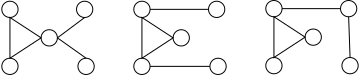
\includegraphics[width=\textwidth]{fig1.pdf}
  \caption{The graph $P_{2\times n}$.}
  \label{fig1}
\end{figure}
We can now tell that no matter how much we extend it, we will always have $6$ cases where two opposite (lower and upper) are colored differently and we have no choice. In the rest of the cases, we will have two options for the last one. We can write this as a recursion for $n\geq 3$:
$$
T(n)=2(T(n-1)-6)+6=2T(n-1)-6
$$
where $T(n)$ is the number of edge colorings of the graph $P_{2\times n}$ and $T(2)=18$. With a little thinking and help of a website\footnote{http://oeis.org/}, we can find a closed form for $T(n)$ when $n\geq 2$:
$$
T(n)=3(2^n+2)
$$
and with the special case where $T(1)=3$.

\section{Problem 5}
Generally, the topics we covered were useful and most of it was actually very interesting. Only thing I really have to say is that I enjoyed the introduction of theorems or topics in form of a problem, e.g. like art gallery problem. There were some topics that required an understading of another topic, e.g. topology, which was took a little more time to understand as a computer scientist as I have never had a course covering that. But it was small things like this and was very easy to survive. \\
On a sidenote, I found the lectures great! The lecturer understood the students well, in the sense that he paused when there were details that were a little harder. Generally, the atmosphere was great during the lectures. Not much to say about the exercise classes, since they pretty much worked as in any other course. The exercise class where Sage was introduced was a little redundant, but again, depending on what background you have, some might have benefited from this. All in all, great course!

\end{document}
